\chapter{Methodology}
This section describes how the results were achieved. The overview figure \ref{MethodologyFigure} presents the proceeding steps.

\begin{figure}
\centering
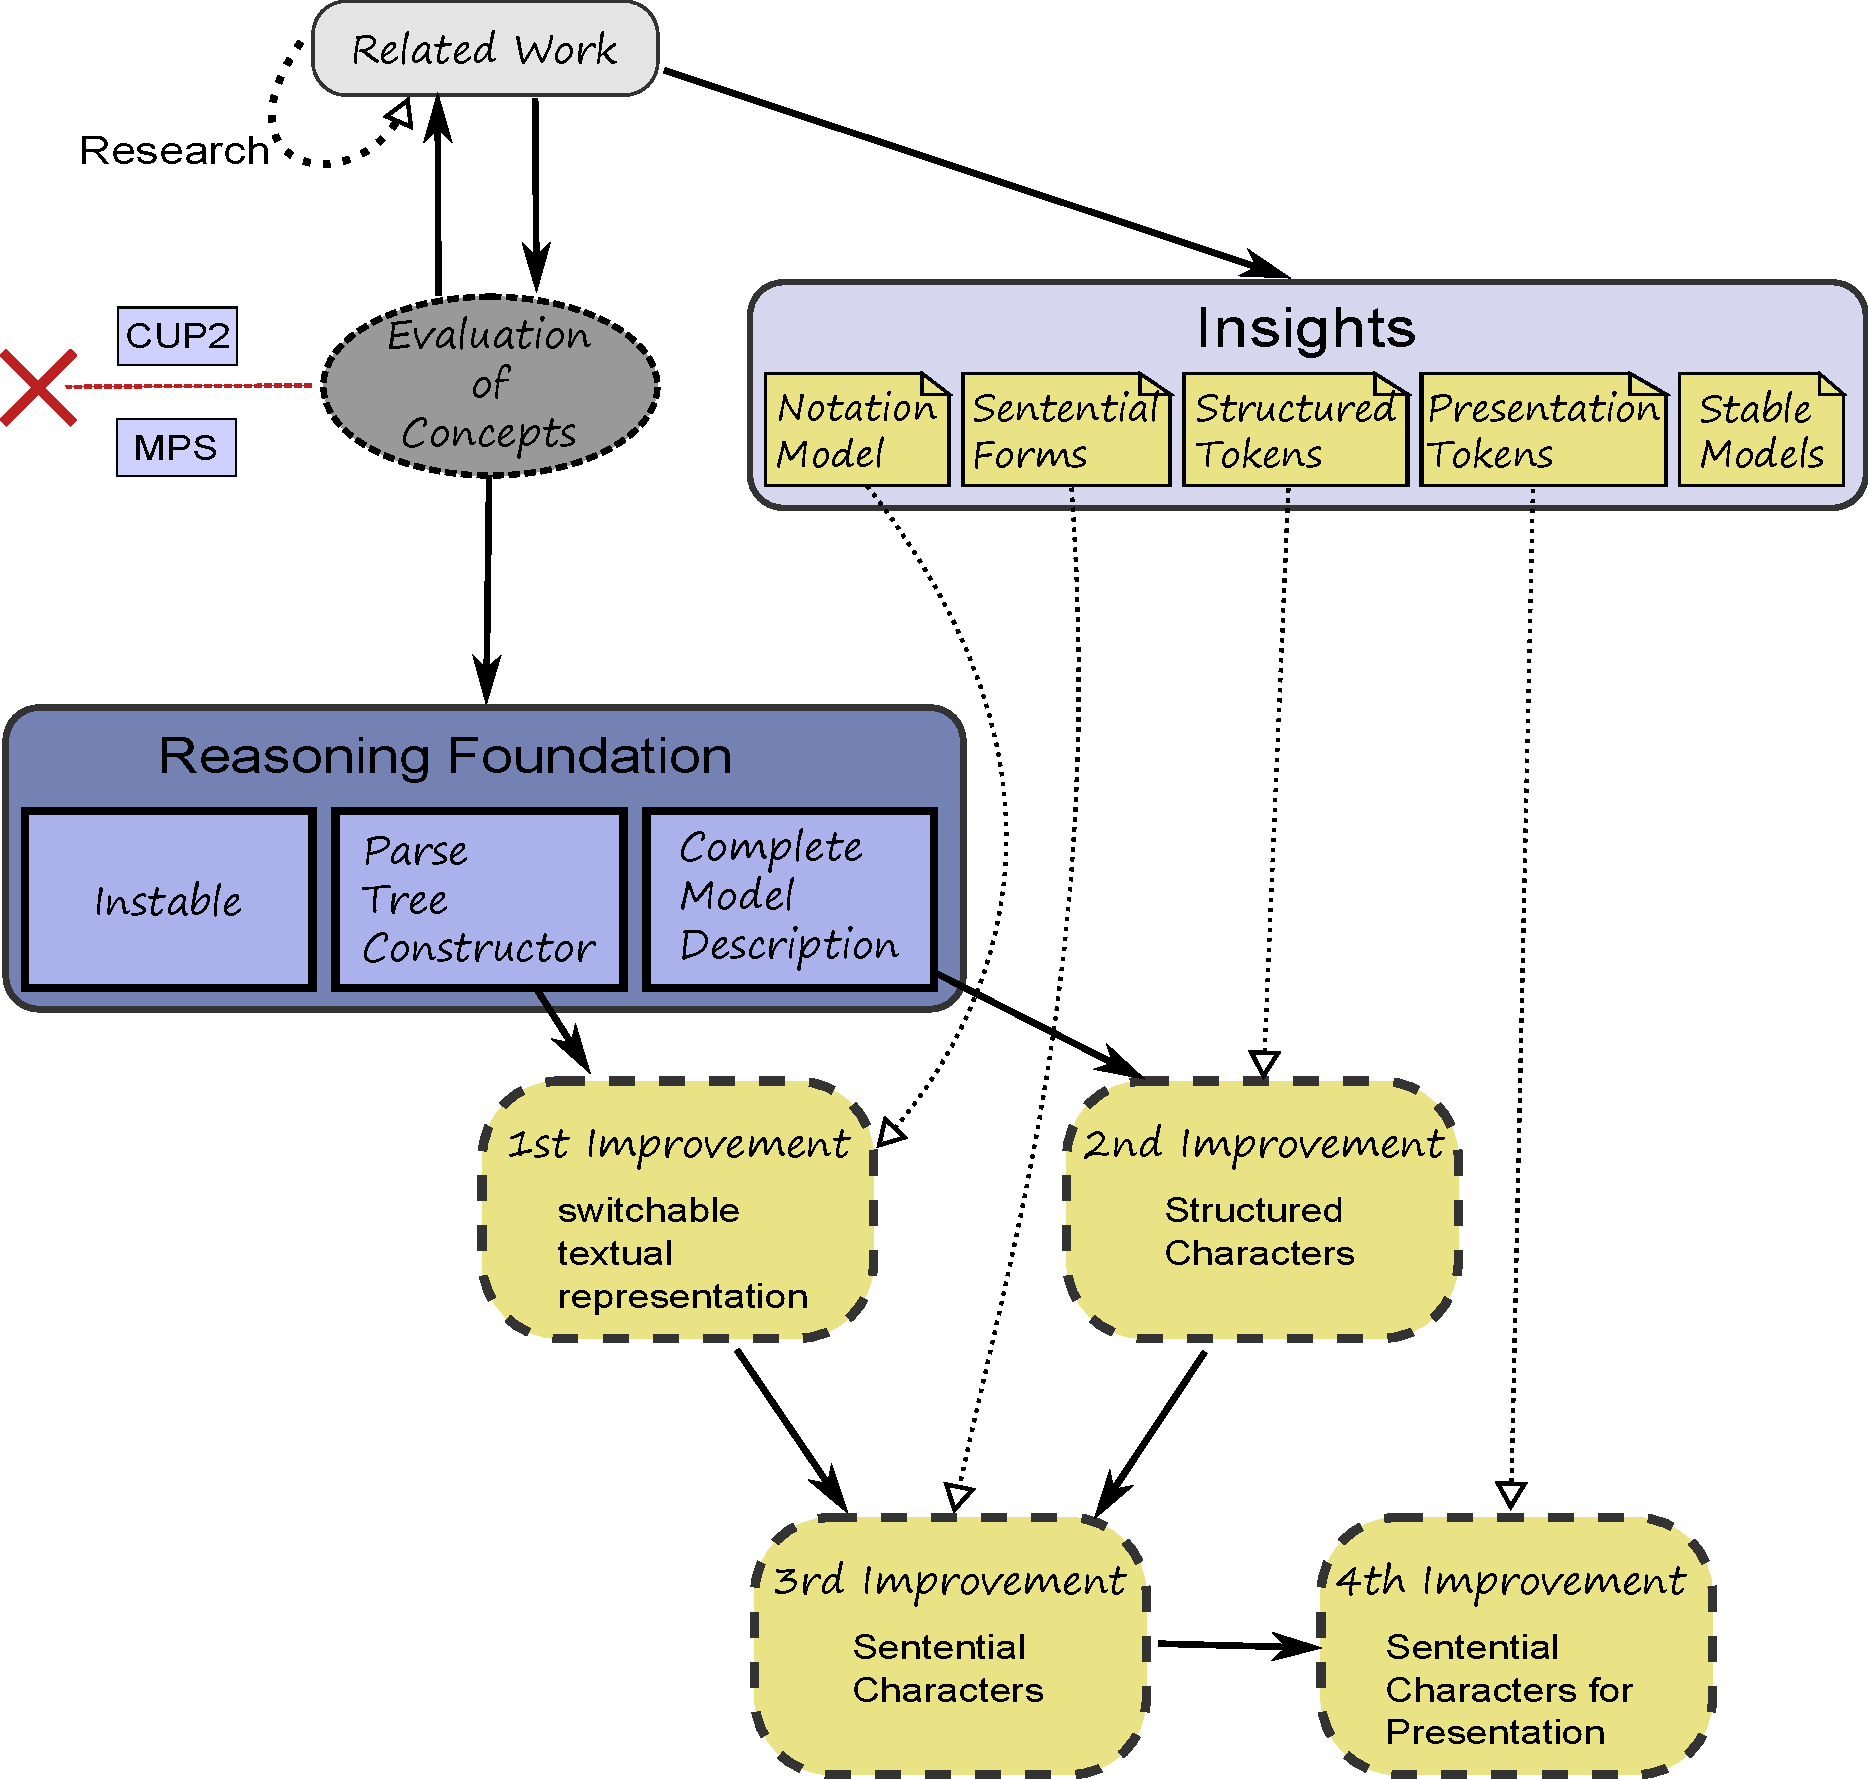
\includegraphics[scale=0.47]{gfx/ex/Concept2} 
\caption{Methodology Overview}
\label{MethodologyFigure}
\end{figure}

The following observations during research were made:
\begin{itemize}
	\item Every non Metamodel based tool uses its own, specific approach for abstract language data structure transformation, validation, persistence and editing.
	\item In the Graphical Modeling Framework (GMF), the \emph{Notation model} generically encapsulates the state of the visual representation.
	\item After a short evaluation of Meta Programming System (MPS), the restricted usability of \emph{projectional textual editing is undesirable} for the target of this thesis. The text editing concept of MPS is template or form based, not free textual. This concluded in additional research.
	\item The CUP2 \footnote{\raggedright \url{http://www2.in.tum.de/~petter/cup2/}} Parser generator framework was evaluated to enable the direct use of \code{EObject}s in the Parser. The insight, that Structured Tokens and thus \code{EObject}s as tokens are valid, led to the abandoning of CUP2. 
	\item Proxima uses a \emph{Structured Token for graphical presentation}, but does not allow it to be directly edited.  Its seven layer architecture with bidirectional model transformations between each allows high flexibility. Dependant layers were considered undesirable, especially regarding possible user interaction on different layers, with the complexity to maintain bidirectionality by two unidirectional transformations and updating instead of replacing model elements. Several model transformation languages for EMF exist, so structural transformations are possible and separated if required. 
		\item Harmonias incremental parsing algorithm for GLR parsing requires the parser to handle \emph{sentential forms}.
		\item The report \cite{Barista} about Barista shows the successful use of a variant of Harmonias incremental parsing algorithms in projectional editors to achieve \emph{stable abstract data structures}.
\end{itemize}


The Xtext framework was evaluated afterwards in regard to add alternative representations.
The following central perceptions were made:
\begin{itemize}
	\item The used, non incremental parsing technology results in unstable models. This characteristic is not considered until its impact on the solution in chapter \ref{cha:discussion} discussion.
	\item The grammar must completely describe the model. 
	\item There is no isomorphism from grammar production to \code{EObject}, which means multiple representations of the same \code{EObject} are possible.
	\item The Parse Tree Constructor determines the production used for model to text transformation. Different textual representations are already possible, but are not accessible by the user or language designer. \\
\end{itemize}

Due to problems with model stability and the gained insights of extensive research, the argumentative deductive approach was chosen for this thesis. The perceptions made for the Xtext framework are used as the reasoning foundation. 

The first conceptional improvement of this thesis allows \emph{switchable textual representations}. This has been solved by extending the Parse Tree Constructor and introducing a Notation Model.\\

\emph{Structured Tokens} highlighted the usage of nested structured data as tokens, which triggered the second improvement. To integrate Structured Tokens in a textual serialization, a Structured Character concept was developed that enables the use of \code{EObject}s as atomic characters on the character stream. \\

The Notation Model developed for the first improvement and the possibility of Structured Characters by the second, together with grammar post-processing enables Sentential Characters. \\

The forth improvement of omitted Parse Subtree construction enhances Sentential Characters for presentation purposes.
